
\chapter{Merchant}
This thesis proposes a merchant software agent that can compete against competition on an online marketplaces.
The merchant makes ordering and pricing decisions with the goal to maximize the profit.
The merchant uses demand learning to estimate future customer demand from historical market situations and sales data.
The estimated demand is used in a dynamic programming approach to generate ordering and pricing policies.
%what is a policy?

We developed the merchant in four phases to overcome the complexity of this problem.
The first phase constrained the merchant's problem the most and only considers the inventory problem with known customer demand in a monopoly.
Each following phase adds a new difficulty for the merchant until the fourth phase which represents our final problem: The joint inventory and dynamic pricing problem with unknown customer behavior under competition.

Each of the following sections explains one phase in detail.
\todo{explain each ''step'' short in some sentences each with references to chapter} \cref{section:ordering}.
%explain structure of following sections

\section{Ordering}
\label{section:ordering}
In this scenario, the merchant cannot make pricing decisions.
Instead, all products are sold to a fixed price.
The merchant can focus on the ordering problem and make ordering decisions that promise the most expected long-term profit.
The merchant has a monopoly and does not have to care about any competitor.
Ordering decisions depend on the customer demand.
The demand is stochastic and its distribution is known to the merchant.
There are no backlogs. %sentence to short?
If a customer arrives when the merchant is out of stock, the merchant will miss the sale.

\subsection{Model Description}
\label{subs:ordering_model}
%situation
%todo more intro/situation
The merchant wants to sell items on the marketplace.
% price & revenue
Items are offered at a fixed price $a_{fix}$ and each sold item generates a revenue of $a_{fix}$.
% time horizon
% write about t here?
The time horizon is infinite.
% discrete time
Since in real-life applications prices cannot be adjusted arbitrarily often, we use a discrete time
model.
%discounting
We use discounting to increase the relevance of short-term profits.
A discount factor $\delta$, $0 < \delta \leq 1$, is applied to each time period.

% inventory + holding cost
%todo introduce time and periods before that
The merchant holds items in an inventory.
The random inventory level at the start of period $t$ is denoted by $N_t$.
Storing items in the inventory causes holding costs of $l$ per item per time period. % l > 0

%ordering
The merchant can reorder items to increase the inventory level.
Order decisions, which can be made once each time period, will influence the merchant's profit.
The number of items ordered at time $t$ are denoted by $b_t$, with $b_t \geq 0$.
A order of size $b_t = 0$ means that no order is made.
%todo order delay
%set depends on time, yes? no?
The set of admissible orders quantities is denoted $B_t$.
% order cost
% explain fixed/variable order cost? explain somewhere else?
Each order causes a order cost, which consists of fixed order cost $c_{fix}$ and variable order cost $c_{var}$.
%order costs paid upfront
Order costs are defined by:

\begin{equation}
\label{eq:order_cost}
C(b) := \begin{cases}
	c_{fix} + c_{var} \cdot b  & \quad \text{if } b > 0 \\
	0  & \quad \text{if } b = 0
\end{cases}
\end{equation}

%sales
The probability to sell $i$ items is denoted by $P(i)$.
%check: myopic somewhere mentioned and explained
Note, that the probability is time-independent because of the consumer's myopic buying behavior.
Additionally, the probability in this scenario is independent from offer prices because the merchants sells in a monopoly with a fixed price.
The random number of sold items within the period $(t-1, t)$ is denoted by $X_t$.
%check: backorders mentioned in previous section
%can I express the line below with random variables?
The merchant cannot sell more items than the inventory holds, i.e. $N_t \geq X_{t+1}$. % use specific n

%whats ordering strategy?
%how to write the policy?
Depending on a given ordering policy $(b_t)_t$, the random accumulated profit from time period $t$ is:

%can I do inf sum here? or switch to avg profit?
$$
G_t := \sum_{s=t+1}^{\infty} (\delta^{s-t} \cdot (a_{fix} \cdot X_s - l \cdot N_{s-1} - C(b_{s-1}(N_{s-1})))
$$

The objective is to find a ordering policy that maximizes the expected total profit $E(G_0 | N_0)$.

% end of model descripiton, maybe write what comes next
%Sales decrease the inventory level over time and orders increase it.

\subsection{Solution Approach}
%why use dyn prog? -> optimal; why optimal?

%what? -> dyn programming
In this section, we want to derive optimal ordering policies.
% with and without delay
We use the dynamic programming approach to find the best expected profit of the stochastic control problem.
% is n defined?
The recursive value function $V_t(n)$ describes the best expected profit $E_t(G_t | N_t)$.
Since this this value function cannot be calculated over an infinite time horizon, we introduce the end time $T$ so that $t = 0, 1, 2, ..., T$.
If $T$ is sufficiently large, $V_t$ converged enough in order that the optimal ordering policy is not affected.
%V_T = 0

$N_{max}$ denotes the upper limit of the inventory level and the order decision, $0 \leq n, b \leq N_{max}$. This does not affect the optimal solution as long as $N_{max}$ is greater than the biggest inventory level that can occur in the optimal policy.

The value function with an instantaneous arrival of orders is:
%where comes i from?
% solve infinite sum over i problem: upper limit, rest probability for i >= n
\begin{equation}
\begin{split}
V_t(n) = \max_{b \in B_t} \Bigg\{
\sum_{i \geq 0} \Big(
P(i) \cdot (
a_{fix} \cdot min(i, n + b) %sales
- l \cdot (n + b) % holding cost
- C(b) % order cost
) \\
+ \delta \cdot V_{t+1}\big(min(max(n + b - i, 0), N_{max}))\big)
\Big)\Bigg\}
\end{split}
\label{eq:dyn_prog_no_delay}
\end{equation}

%check: order delay mentioned in model description?
Solving this problem with any order delay results in a huge increase in dimensions for the calculation.
The computation time would be to long to make fast and dynamic decisions on an online marketplace.
To avoid these long computation times, we assume that the order delay is exactly one period.
This solution is a heuristic for different order delays.
The value function with order delay is shown in the following equation:

\begin{equation}
\begin{split}
V_t(n) = \max_{b \in B_t} \Bigg\{
	\sum_{i \geq 0} \Big(
		P(i) \cdot (
			a_{fix} \cdot min(i, n) %sales
			- l \cdot n % holding cost
			- C(b) % order cost
		) \\
		+ \delta \cdot V_{t+1}\big(min(max(n - i, 0) + b, N_{max}))\big)
	\Big)\Bigg\}
\end{split}
\label{eq:dyn_prog}
\end{equation}

The set of order quantities $B_t$ must contain zero to allow to make no order.
The optimal ordering policy $b_t^*(n)$ is given by the arg max of \cref{eq:dyn_prog_no_delay} and \cref{eq:dyn_prog} respectively.
%address that arg max is set, do that in next sections too
The next sections will only consider the case with delayed orders.

\subsection{Evaluation}
%konvergieren der wertefunktion
%vergleiche mit startwert 0, gleicher wert, zu hoher wert
%wie schnell konvergiert es (konvergiert es)? welchen einfluss hat der startwert?
\todo{show graph of converging value function}

%told, that this is a optimal ordering policy
%deviations from that should result in worse performance (profit)
%let's compare computed optimal policy in monopoly with policy that orders one item more(less)
%hint: use bigger dif if you cannot see difference in policies
\todo{compare with merchant that buys always one more / one less}

\section{Joint Ordering and Pricing}
\label{section:joint_ordering_pricing}
%What?
In this section, the merchant is in the same situation as in \cref{section:ordering} but additionally gains control over the selling price.
With ordering and pricing decisions enabled, the merchant's actions on the marketplace are unconstrained.
%Difference in demand
The demand in this scenario depends on the chosen selling price.
A higher price usually results in less demand.
As in the previous problem, the demand distribution is known.

%Why joint:
We cannot separate the inventory and pricing problem and solve each in isolation to solve the whole problem optimally.
Ordering and pricing decisions influence each other.
Setting a price changes the demand, which requires a different ordering policy.
The other way around, an ordering policy might require certain prices for a better control over inventory levels.
This mutual influence is the reason, why ordering and pricing should be decided jointly.

\subsection{Model Description}
\label{subs:joint_model}
This model is a extension of the model from \cref{subs:ordering_model}.
%pricing decision
Instead of a fixed selling price $a_{fix}$, the merchant sets a price $a_t$ in each period $t$, with $a_t \geq 0$.
The set of admissible pricing decisions is denoted $A_t$.
%revenue
Each sold item in period $t$ generates a revenue of $a_t$.

%demand
The probability to sell $i$ items depends now on price $a$.
The merchant knows the price-dependent probability distribution.

Depending on a given pricing and ordering policy $(a_t, b_t)_t$, the random accumulated profit from time period $t$ is:

% can i reuse name from previous section?
$$
G_t := \sum_{s=t+1}^{\infty} (\delta^{s-t} \cdot (a_{s-1} \cdot X_s - l \cdot N_{s-1} - C(b_{s-1}(N_{s-1})))
$$

The objective is to find a joint pricing and ordering policy that maximizes the expected total profit $E(G_0 | N_0)$.

\subsection{Solution Approach}
\label{section:joint_solution}
As a basis, we use the dynamic programming approach shown in \cref{eq:dyn_prog}.
The Bellman equation is extended by one dimension that contains all pricing decisions $A_t$.

%todo remove t from A and B.
\begin{equation}
\begin{split}
V_t(n) = \max_{\substack{b \in B_t \\ a \in A_t}} \Bigg\{
\sum_{i \geq 0} \Big(
P(i, a) \cdot (
a \cdot min(i, n) %sales
- l \cdot n % holding cost
- C(b) % order cost
) \\
+ \delta \cdot V_{t+1}\big(min(max(n - i, 0) + b, N_{max}))\big)
\Big)\Bigg\}
\end{split}
\label{eq:dyn_prog_joint}
\end{equation}

There are three changes to the value function.
The probability is price-dependent ($P(i, a)$), the revenue in one period depends on the chosen price ($a \cdot min(i, n)$), and the maximum expected profit over all ordering decisions and pricing decisions is used.
The optimal ordering policy $b^*_t(n)$ and pricing policy $a^*_t(n)$ are given by the arg max of \cref{eq:dyn_prog_joint}.
%optimal pricing decision

\subsection{Evaluation}
\todo{show policies with increasing prices}
% anything else I can show here?

\section{Demand Learning}
\label{section:demand_learning}

This section extends the joint inventory and dynamic pricing problem from \cref{section:joint_ordering_pricing} by not providing the merchant with the demand distribution.
%the merchant, the merchant, the merchant...
The merchant needs to know the customer behavior in order to make effective ordering and pricing decisions.
The merchant can get information about the customer behavior from past customer actions.
The merchant can analyze historical market situation and sales in order to deduce future customer behavior.
%what is this dat, where is it from? (how does it look like?)
This is called demand learning.

%from data to demand distribution

%model section removed, maybe mention somewhere that problem is same, only prob is not know

\subsection{Solution Approach}
In order to overcome the inventory and dynamic pricing problem with missing demand information, we split the whole problem into two parts.
The first part is the training of a model from historical market situations and sales in order to predict sale probabilities.
These probabilities are used in the second part to create ordering and pricing policies.
%why sales prob = demand prob? check whole section
Given predicted sale probabilities, the dynamic programming solution from \cref{section:joint_solution} can be used as it is, to calculate ordering and pricing policies.

Assuming, the merchant predicts the demand correctly, the result will optimal policies.
In other cases, the quality of policies will depend on the quality of predictions. 
The separation of the problem let us focus on the prediction of the demand probability, while having a working solution for the policy creation.

%bring data into right form
In order to to use market and sales data for demand learning, it must be transformed into a usable form.
From the market data we know, at what times the market situation changed and what the market situation was.
The sales data contains information about all of a merchant's sales, including when the sales happened.
These two data sources can be combined and aggregated to a form that contains the number of sales per minute for each market situation.

%bring data into right form, part 2 feature extraction
We use regression analysis for the demand learning.
Regression analysis models and analyzes the relationship between a dependent variable and independent variables.
In this case, the dependent variable is the sales per minute metric.
Independent variables are extracted from the market situation.
In the monopoly scenario, the demand depends only on the merchant's price.
That is why for now, there is only one independent variable, the selling price.
%motivation: why use linear regression and not something else? is relationship linear?
We use linear regression to find a relationship between the independent variables $\vec{x}$ of a market situation and the sales per minute $\hat{y}$ for this situation.
The following equation shows how to predict sales per minute $y$ for a market situation.

%show how x is vector of features and constant 1 \begin{pmatrix} 1 \\ p \end{pmatrix}
\begin{equation}
\label{eq:linear_regression}
y = \vec{x}^\intercal \cdot \vec{\beta}
\end{equation}

$\vec{\beta}$ consists of the weights of the regression model.
Given the sales per minute $y_1, y_2, \ldots, y_n$ and the independent variables $\vec{x}_1, \vec{x}_2, \ldots, \vec{x}_n$ from $n$ historical market situations, the weights $\vec{\beta}$ are calculated with the least squares approach:

%todo fix on https://en.wikipedia.org/wiki/Linear_regression, ask Rainer
\begin{equation}
\vec{\beta} = \bigg(\sum_{i=1}^n{\vec{x}_i \vec{x}_i^\intercal} \bigg)^{-1}
			  \bigg(\sum_{i=1}^n{y_i \vec{x}_i} \bigg)
\end{equation}

%predicted mean demand -> distribution
The merchant is able to predict mean sales per minute for a market situation with the regression analysis.
However, sales probabilities are needed for the dynamic programming approach.
The mean sales per minute can be used as a parameter to create a probability distribution.
%find better citation with a study or something to show that.
We describe the demand distribution with a Poisson distribution.
This discrete distribution is a good approximation for the arrival and buying process of customers \cite{DBLP:journals/ior/Wolff82}.
Equation \ref{eq:probability} shows to integration of the Poisson distribution and the linear regression from \cref{eq:linear_regression} in order to create a demand probability function.

\begin{equation}
\label{eq:probability}
P(i, \vec{x}) =
	e^{\frac{-1}{\vec{x}^\intercal \vec{\beta} \cdot p}}
	(\vec{x}^\intercal \vec{\beta} \cdot p)^{-i}
	\frac{1}
	{i!}
\end{equation}
%todo fix ugly transpose

$p$ is the length of the merchant's decision period in minutes and $p > 0$.
The sales per minute are multiplied with the period length to get the number of sales in a period.
This demand probability function is used in \cref{eq:dyn_prog_joint} to calculate order and pricing policies without knowing the demand distribution.

%retraining
The merchant has access to a steadily growing collection of market situations and sales data over time.
The quality of predictions is increased by periodic trainings that utilize the new data.
There is no trainings data available at the start of a merchant's career on the marketplace.
In that case, we use a rule-based ordering strategy and an exploration pricing strategy.
The exploration pricing strategy sets random prices.
This allows the merchant to encounter many different market situations and obtain sales data for these situations.

\subsection{Evaluation}

\todo{show how good predicted percent to real percent is}


\todo{show prediction quality over number of training examples}

\section{Competition}
Until now, the merchant offered items on the marketplace in a monopoly.
This is usually not the case on real online marketplaces.
Other merchants offer the same or similar products and everyone wants to make the most attractive offer.
A common strategy to do that is to offer the cheapest price.
When multiple merchants pursue this strategy, the price will spiral downwards.
Such a commercial competition is called price war.
It is not the best strategy to always undercut the competitors because of decreasing profit margins.
Sometimes it is better to offer a higher price.
This reduces sales, but the profit margin is higher.
This section proposes a merchant that makes optimized ordering and pricing decisions under competition with the goal to maximize profit.

In the previous sections, the sale probability was only influenced by the merchant's own actions, to be specific it was influenced by the selling price that the merchant sets.
In this scenario, the merchant's sale probability is also influenced by competitor's actions.
%model description
The model is the same as in \cref{subs:joint_model} with the exception that number of sold items $X_t$ within a period depends on the merchant's offer price and the competitor's offer prices.
Merchants have access to historical market and sales data.
The sales data contains only information about a merchant's own sales, not the sales from the competitors.

%merchant must be fast
Market situations can change frequently on online marketplaces.
A merchant must able to quickly and effectively react on new market situations in order to offer an optimal price for the new situation.
Getting fast decisions is a challenge because the increasing complexity of the inventory and dynamic pricing problem over the last sections resulting in solutions with increasing computational effort.
Nevertheless, there are ways to improve the speed of the dynamic programming approach which are described in \cref{section:faster_dyn_prog}.

\subsection{Solution Approach}


%build on top of solution from previous section


%describe two possible approaches
%todo reread, and split paragraph
The inventory level was the only state on which ordering and pricing decisions were based on in the previous problems.
With competitors on the marketplace, the merchant must also consider their offers when making ordering and pricing decisions.
One possible approach is to add competitors' offers to the state in the dynamic programming calculation.
We decided against this solution because it drastically increases the state by multiple dimensions and therefore slows the computation down by multiple orders of magnitude.
Moreover, demand learning must predict transitions of competitors' offers from one time period to another.
This means that competitors' strategies must be learned, which requires a substantial amount of trainings data and a complex demand model to make sensible predictions.
Instead, we take the following approach.
We create ordering and pricing policies whenever the market situation changes for that specific new market situation.
The ordering and pricing decisions for this approach depend only on the merchant's inventory level.
This keeps the computation fast and efficient.
Additionally, only sale probabilities are predicted but not the competitors' price reactions.
This can be done by a relatively simple demand model, which can make good predictions even with few market and sales data.
The disadvantage is that new policies must be computed for each new market situation.
The next sections tackles the problem of how to quickly compute ordering and pricing policies for new market situations.

%market situation more complex -> more features
Market situations become more complex with the introduction of competition.
Previously, there was at most one active offer at a time.
Now, there can be as many offers as competing merchant.
And the number of offers can change over time when merchants are out of stock.
In \cref{section:demand_learning}, the merchant's offer price was sufficient to describe a market situation.
With competition, the sale probability of an offer depends not only on its price but also on the price of the other offers.
%todo use everywhere explanatory variables instead independent variable
New explanatory variables are necessary for demand learning to describe the more complex market situations.
We created two new explanatory variables besides the offer price in order to describe market situations with competition.
The variables are explained in detail below.

%todo bold bullet points
\begin{description}
	\item [Own price]
		This explanatory variable hold the value of the merchant's current offer price.
		It helps to explain effects on the sale probability that are based on the total price.
		For example, a higher price generally results in less demand.
	\item [Price rank]
		This variable describes the merchant's relative position in the price ranking.
		The price rank is defined by the number of competitors' offer that cost equal or less than the merchant's offer.
		Demand learning uses this to find a relationship to the sale probability.
		For example, it is probable that a merchant sells more items by having the cheapest offer instead of the second cheapest.
	\item [Price difference to cheapest offer]
		This is the difference in price from the merchant's offer to the cheapest offer.
		If the merchant has the cheapest offer, the variables value will be €0.
		It is a relative variation of the 'own price' metric.
		This variable could explain effects like: a customer is willing to pay €5 more than the cheapest product but not €10 more.
\end{description}

With these explanatory variables it is possible to describe the effect of the competition and the merchant's offer price on the sale probabilities.

The predicted sale probability are used in the dynamic programming approach to compute ordering and pricing policy.
As explained above, the policies are computed for each new market situation.
%todo fix time mentioned
At this point, the computation takes around two seconds to complete.
This is to long for the merchant to quickly and frequently react on the changing market.
In the next section, we will reduce this time to allow shorter decision intervals for the merchant.

%todo dyn progamming formula with p(i,x) in demand section
%todo make x depend on price somehow

\subsection{Efficient Dynamic Programming}
\label{section:faster_dyn_prog}
In this section, we present four approaches to increase the computational efficiency of dynamic programming.
These approaches are applied to our merchant to reduce time spent on computing policies.
This allows the merchant to react faster on new market situations.
The approaches are: using a better start value, adapt decision sets, and tweaking the number of iterations.

%better start value
%todo reference to convergence figure
%todo how to call 'start value', 'end value'?
Figure (...) shows that dynamic programming converges faster if the start value is near the end value.
We assume that the expected profit from two successive market situations is similar because the market situations will not fundamentally change in that short time frame.
%wtf, explain more detailed
Setting the start value to the expected profit from the previous computation will reduce the time until dynamic programming converges.
Even if the assumption does not hold true and there is a big change in expected profit, the computation converges most of the time faster than with the old start value of zero.
%equation with start value

%adapt decision sets
%todo remove t from decision set A and B
%very passiv part
Another way to increase the efficiency of the dynamic programming approach is to change the set of pricing decisions $A$ and set of ordering decisions $B$ to only contain relevant decisions.
E.g., a order quantity of 100 is an irrelevant decision if the final policy only uses order quantities around 10.
The irrelevant decision can be removed from the decision set without affecting the result.
%better name/include for T
The dynamic programming approach is run for a reduced number of periods $T$ for approximations of pricing and ordering policies.
%maybe explain this with min, max
After that, new decision sets are created, containing the range of decisions that occur in the approximated policy.
The ranges are increased by some constant to contain decisions that were not used before.
The new decision sets are used to compute pricing and ordering policies again.
The second dynamic programming computation is faster because it works on a reduced pricing and ordering decision sets.
This process can be repeated in order to adapt the decision sets multiple times.
This approach is not only faster than computing policies on the full decision sets, it also removes the limitation of having a static lower and upper limit on the price and order quantity.
The decision sets can be adapted until they contain relevant decision.
No prior knowledge of relevant prices and order quantities is necessary.
%mention 0 special value for order decisions?
%stop after x iterations or until policy converged
%quantisation (not done here) (range vs stride)

%change number of iteration
The end time $T$ is a parameter that affects the number of iterations and therefore the computation time of the dynamic programming approach.
The choice of this parameter is a trade-off between precision for large $T$ and efficiency for small $T$.
One observation is that the policy converges faster than the calculated expected profit.
This can be used to reduce $T$ without affecting the precision of the resulting policies.
It is possible to further reduce the end time $T$, if approximations of the optimal pricing and ordering policies are sufficient.

%show speed increase, maybe here maybe in eval

\subsection{Evaluation}
\todo{compare speed and result of full dyn programming and more efficient way}
%speed down to 0.1 sec
% fazit: now fast enough for fast reactions

\subsection{Oligopoly Simulation}
This section shows how our merchants performs in an oligopoly.
The merchants sell products on the \pricewars platform.
The objective is to maximize the profit.

%present rule-based merchants
Our merchant, called data-driven merchant, competes with two rule-based merchants.
The cheapest merchant always undercuts competitors in order to offer the cheapest product.
%check: but as high to be still cheapest
The cheapest merchant tries to have the most sales by offering the best price.
This merchant does not have a lower price limit and is willing to undercut competitors down to €0.
The second rule-based merchant, called two bound merchant, undercuts competitors similarly to the cheapest merchant.
However, the merchant has a upper and lower price bound.
If offer prices go below the lower price bound, the two bound merchant raises prices to the upper bound.
Moreover, the upper price bound is the maximum price that this merchant will set.
Both rule-based merchants have a static ordering policy.
They order whenever the inventory level falls below a threshold and order as many items to reach a certain inventory level.

\begin{figure}[t]
\centering
\begin{subfigure}{0.5\textwidth}
\centering
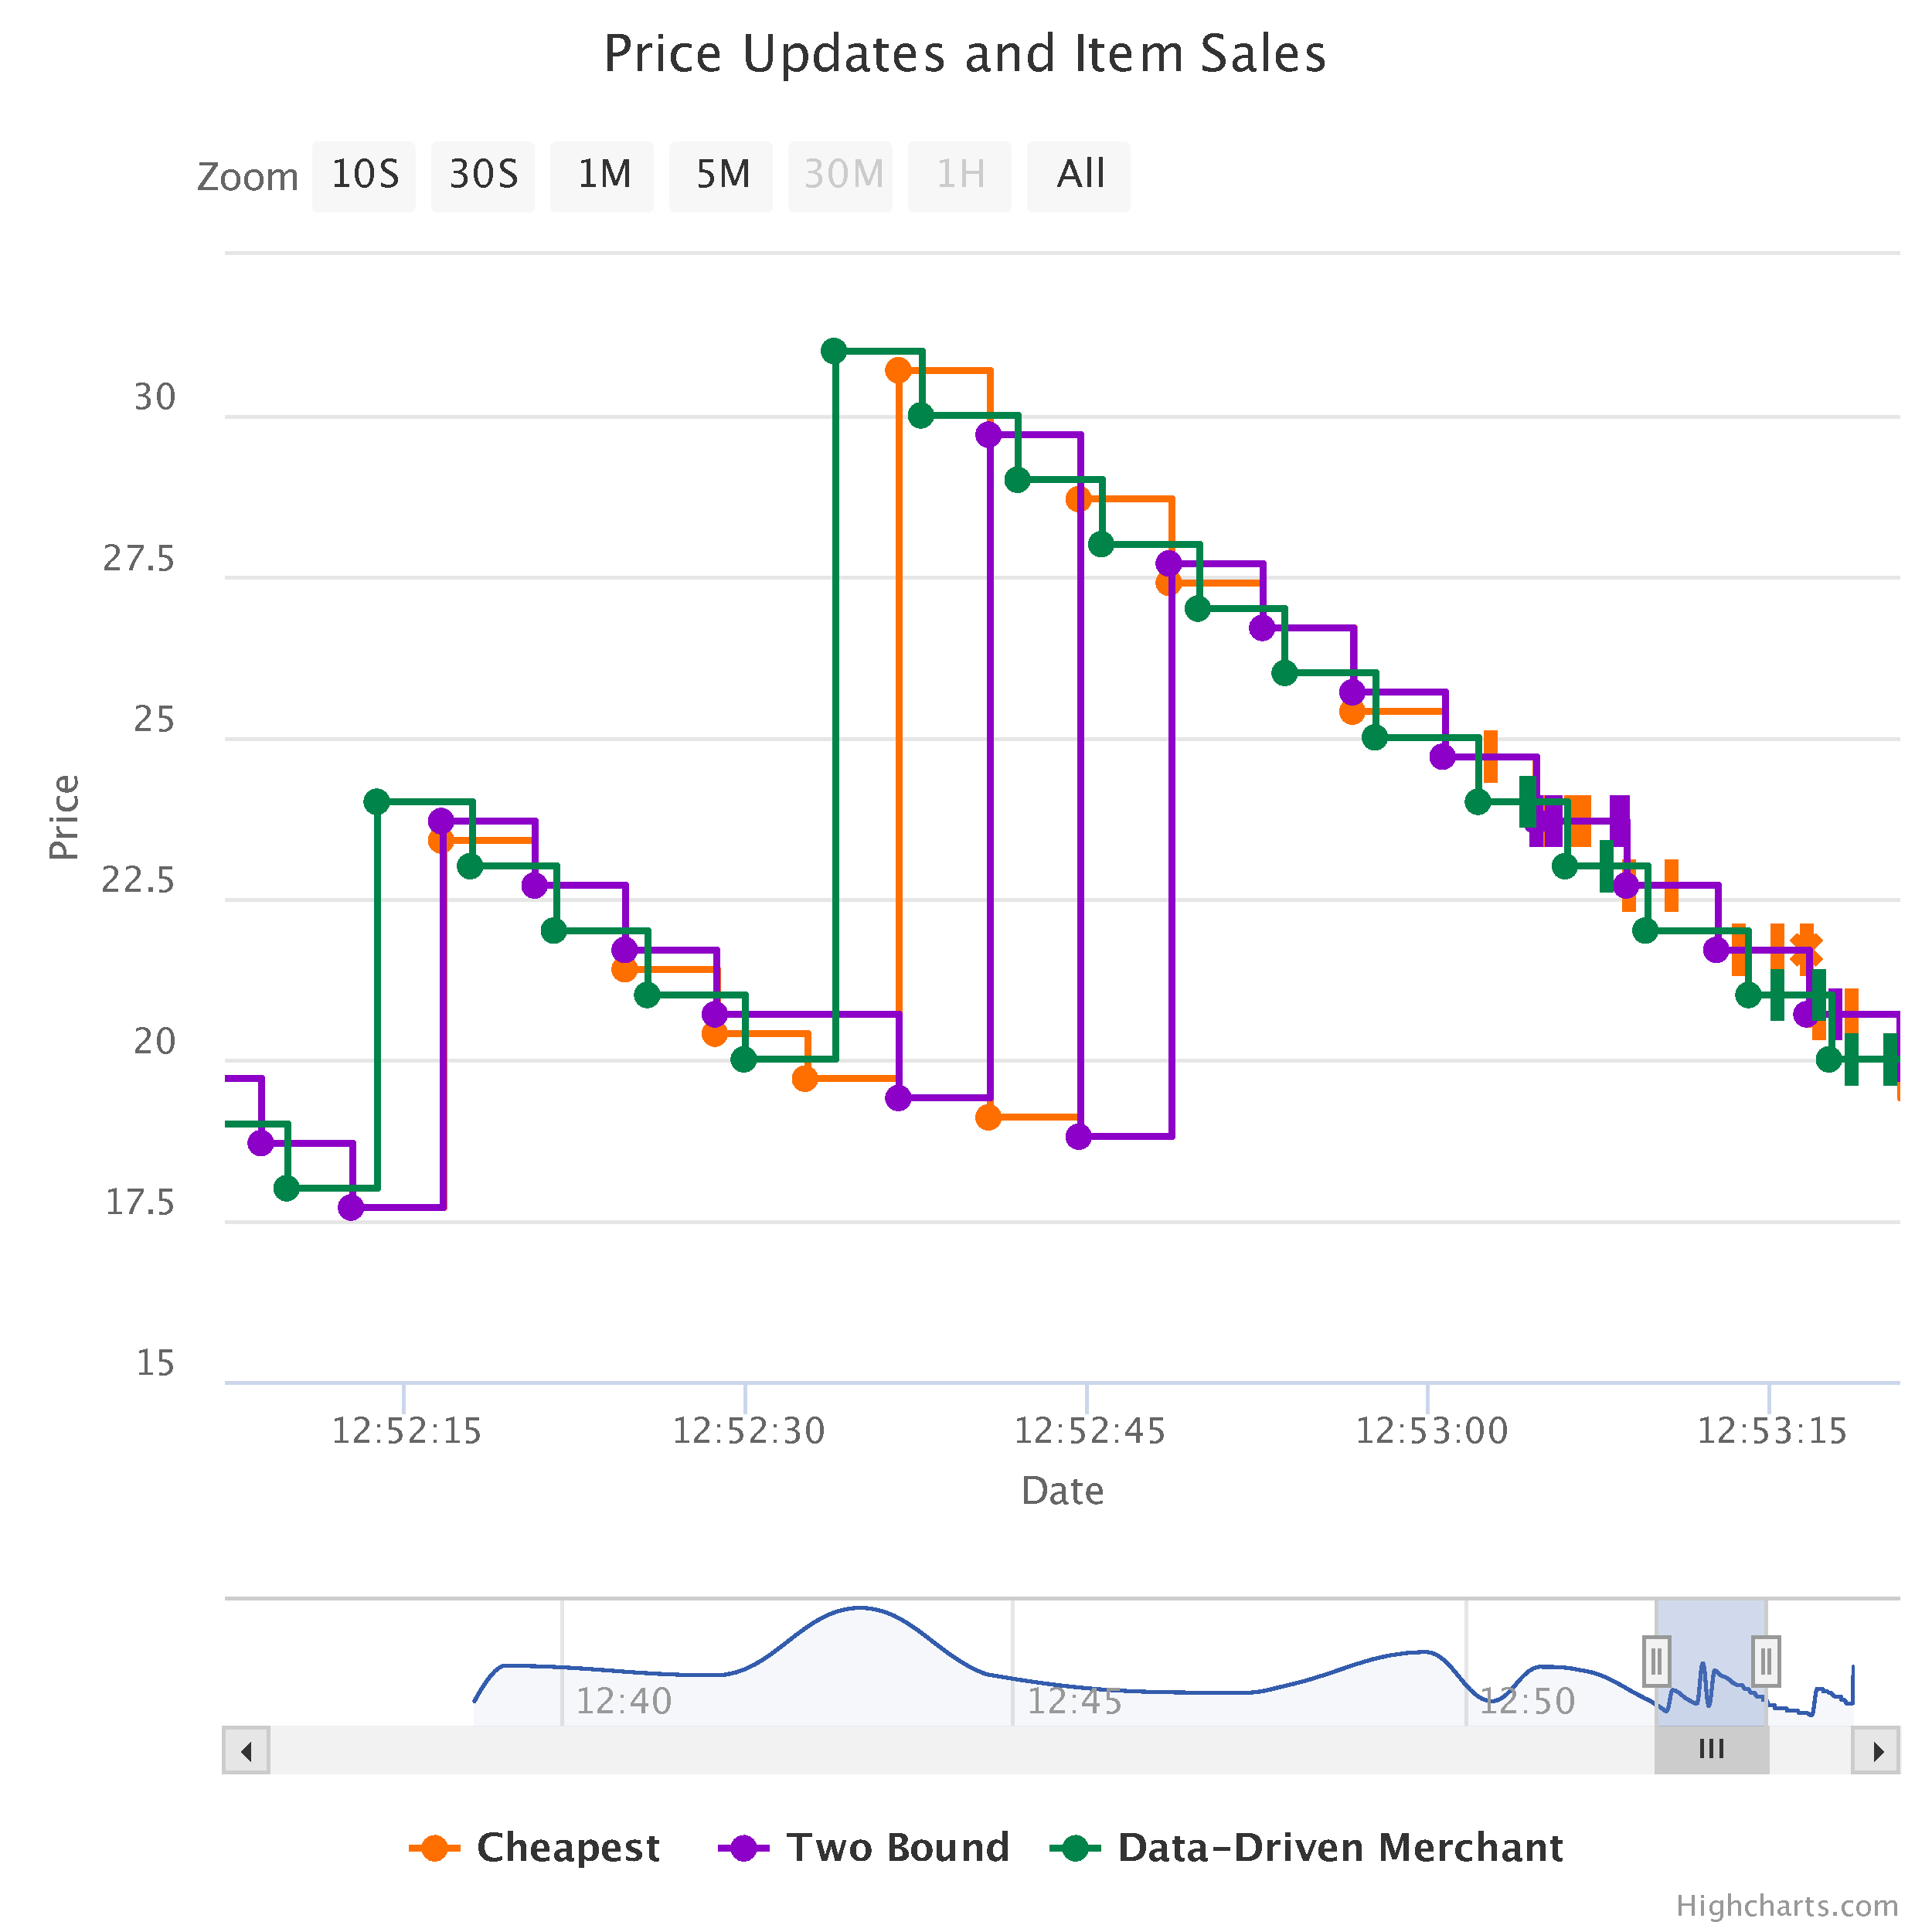
\includegraphics[width=\textwidth]{figures/competition_prices.pdf}
\end{subfigure}%
\begin{subfigure}{0.5\textwidth}
	\centering
	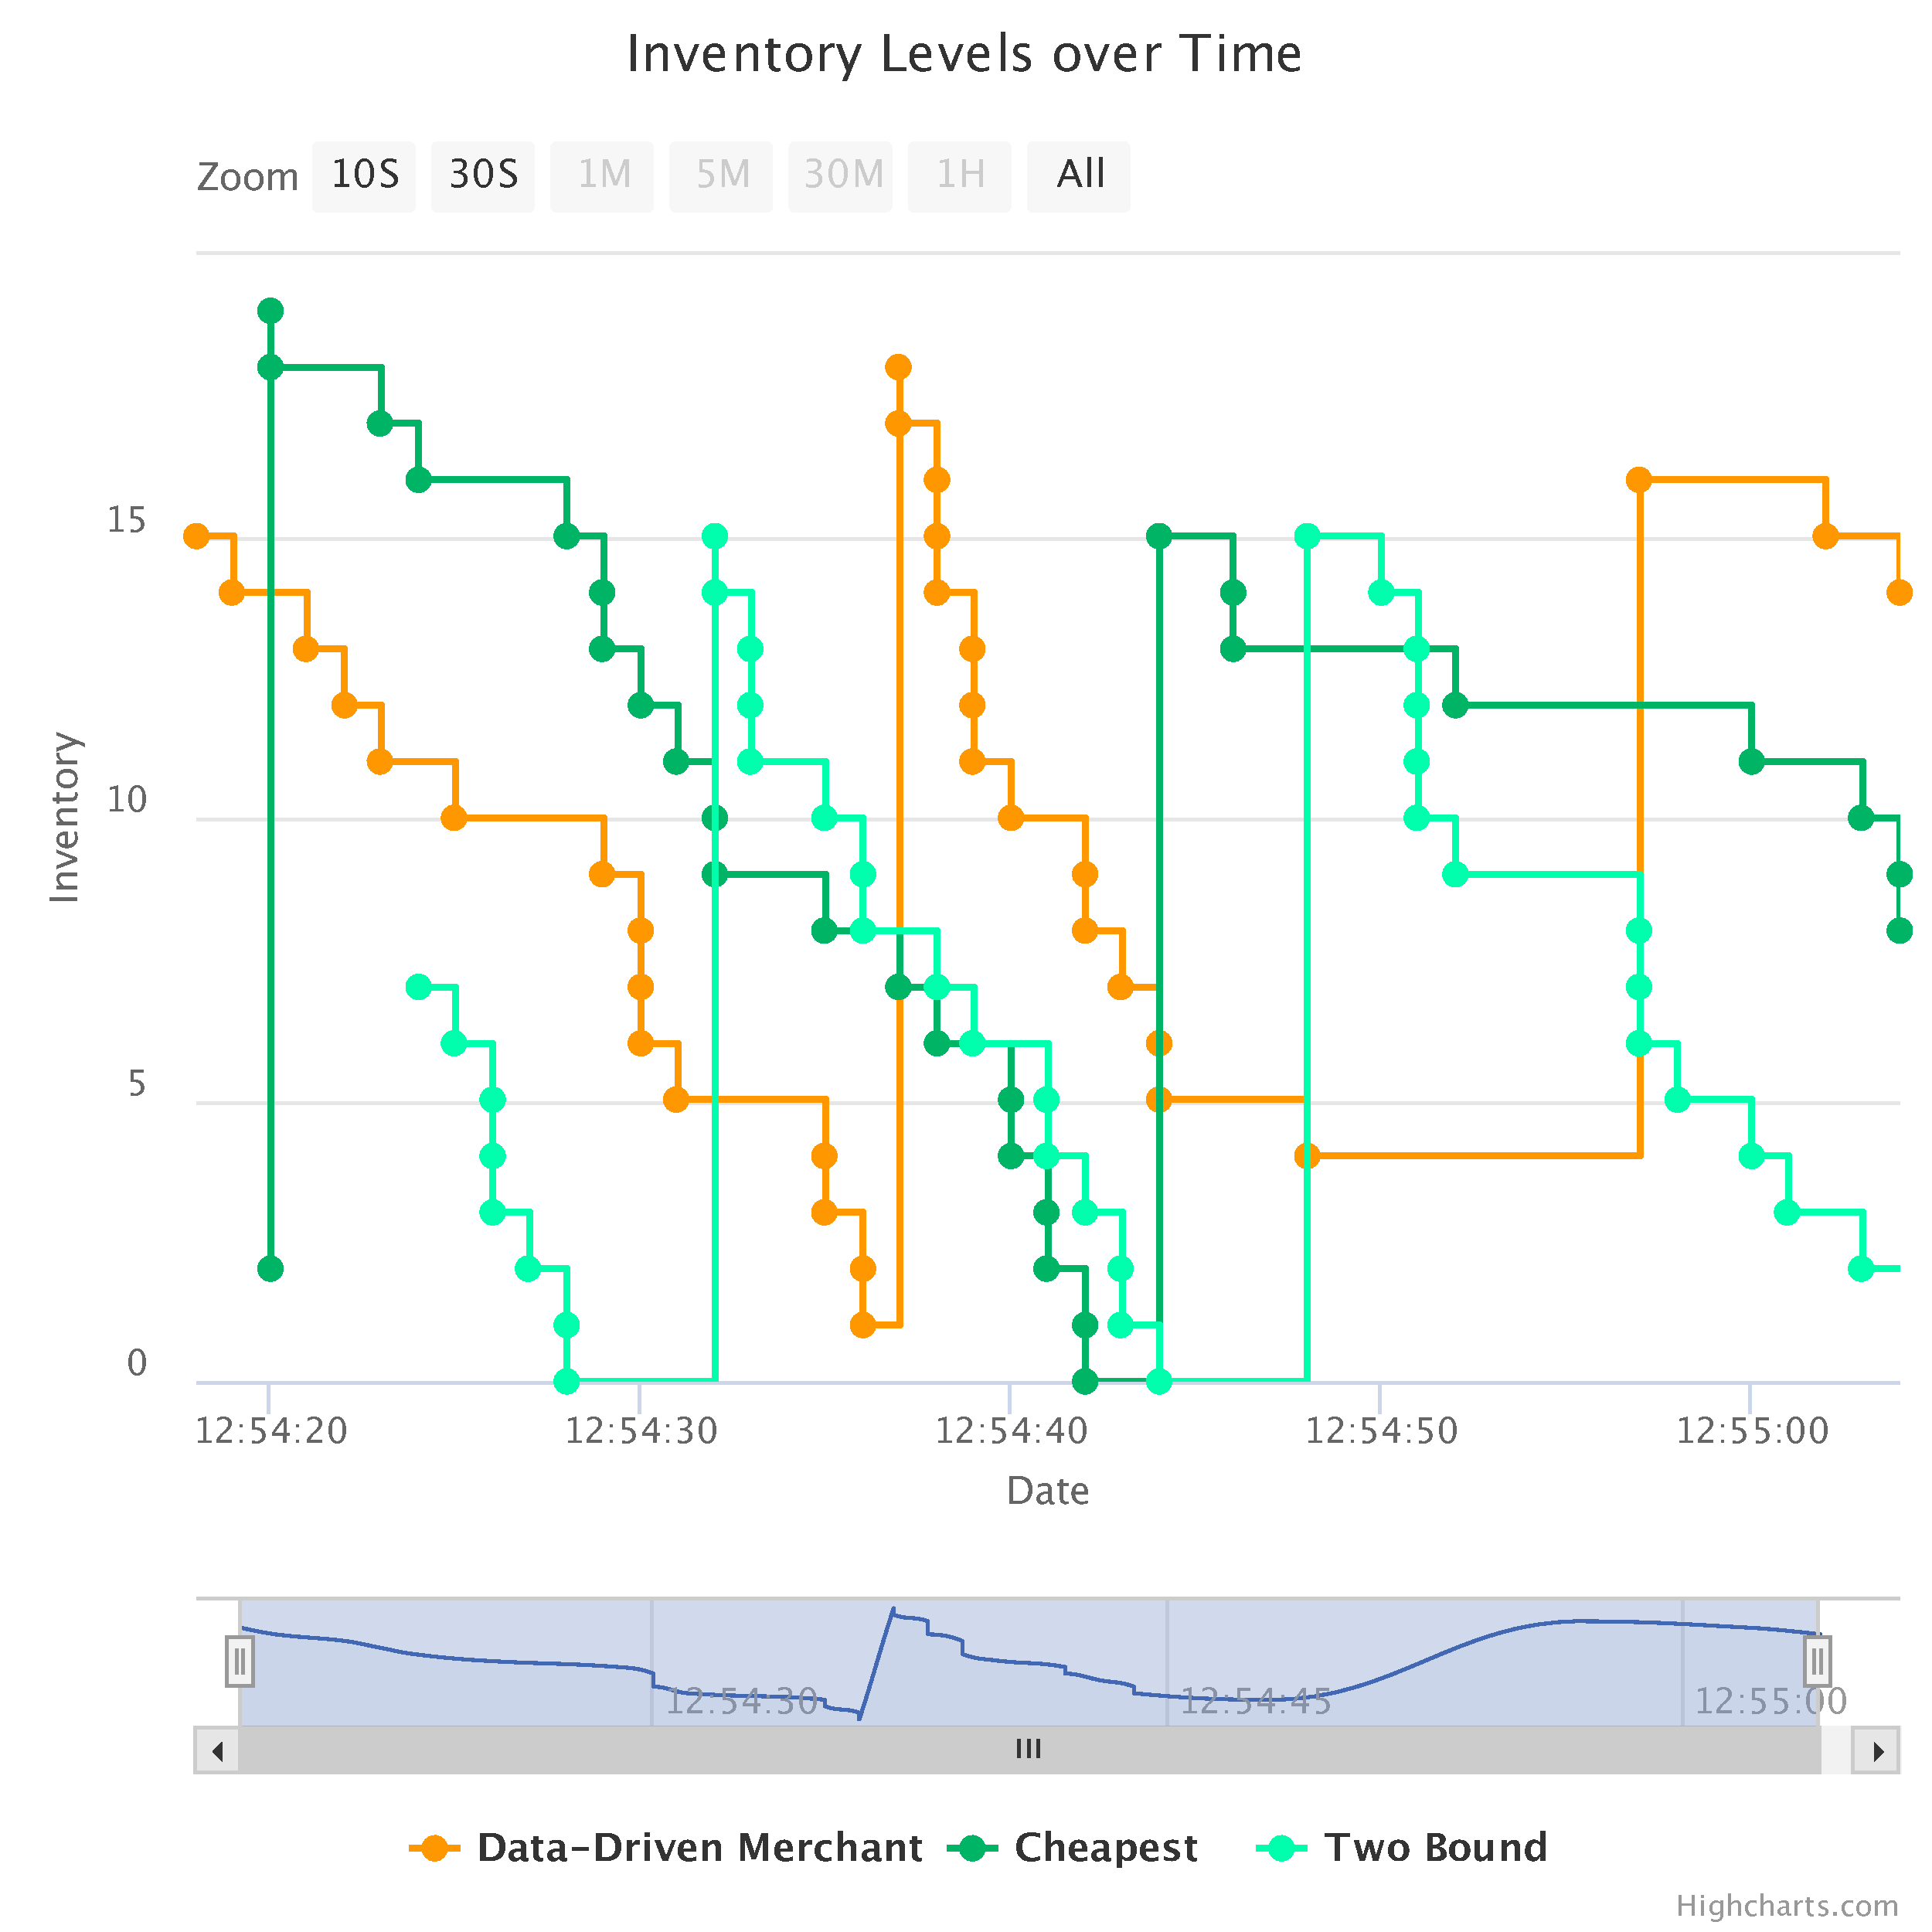
\includegraphics[width=\textwidth]{figures/competition_inventory.pdf}
\end{subfigure}	
	\caption{Price trajectories and inventory levels over time from an oligopoly scenario on the \pricewars platform. Our data-driven merchant competes with two rule-based merchants.}
	%analyze bahavior in one sentence?
	\label{fig:competition}
\end{figure}

We simulated the scenario with competition on the \pricewars platform.
The management UI shows pricing and ordering decisions during the simulation (see \cref{fig:competition}).
The data-driven merchant learned the advantage of undercutting competitors' offers.
However, this creates a price war and offer prices decrease.
With shrinking profit margins, it becomes unprofitable to set the price below competitors' prices.
The data-driven merchant pushes the price up in such a situation.
This action is especially successful if the competitors also increase their offer prices.

\begin{table}[t]
	\centering
	\begin{tabular}{ @{}lrrrr@{} }
		\hline
		& Profit & Revenue & Holding Cost & Order Cost \\
		\hline
		Data-Driven & 5944.13 & 21938.00 & 943.87 & 15050.00 \\
		Cheapest & 5386.90 & 23770.80 & 903.89 & 17480.00 \\
		Two Bound & 5038.63 & 20148.30 & 644.67 & 14465.00 \\
		\hline
	\end{tabular}
	\caption{Simulation results of the oligopoly scenario. The data-driven merchant made the most profit. The cheapest merchant made the most revenue.}
	\label{tab:competition}
\end{table}

\cref{tab:competition} shows the results of a half an hour competition between three merchants.
The data-driven merchant outperformed all competitors.
Our data-driven merchant made around 10\% more profit than the cheapest merchant and 18\% more than the two bound merchant.
Interestingly, our merchant did not make the most revenue, but the cheapest merchant did.
The cheapest merchant sold the most items but with low profit per item.
Our merchant made the most profit by saving a lot of order cost compared the to cheapest merchant.
The data-driven merchant orders on average more items than the competitors.
This results in higher holding costs but saves on fixed order cost.

%command: python3 helper_scripts/benchmark.py -o ../runs -d 30 --merchants "python3 /home/carsten/pricewars-merchant/merchant.py --port 5000 --strategy Cheapest" "python3 /home/carsten/pricewars-merchant/merchant.py --port 5001 --strategy \"Two Bound\"" "python3 /home/carsten/pricewars-merchant/merchant_scenario4.py --port 5002" --holding_cost 3

\todo{show reaction when changing demand or fixed ordering cost}
%

\section{Implementation}
%todo ref python and libs
%how is merchant implemented? (language choice)
Merchants on the \pricewars platform can be written in any language as long as they comply with the platform's REST APIs.
%ref to pytho
We decided to implement our merchant in the Python programming language for the following reasons.
Python has great library support for numerical computing.
These libraries allow a concise and efficient implementation without reinventing the wheel.
The \pricewars platform offers a library written in Python, that implements the APIs to communicate with the platform's services.
Lastly, it is possible to quickly create prototypes in that language.

%architecture
Our merchant consists of four components as it is shown in \cref{fig:merchant_architecture}.
%motivation for this architacture
%main loop
The main loop is the central component.
It regularly checks the marketplace for open offers, updates prices, and orders items from the producer.
After enough time passed, the merchant requests new market and sales data from the kafka reverse proxy and provides it to the demand learning component to analyze demand.

\bgroup
\tikzstyle{block} = [draw, rectangle, minimum height=3em, minimum width=6em]
\tikzstyle{pinstyle} = [pin edge={<-,thin,black}]
\tikzstyle{rpinstyle} = [pin edge={->,thin,black}]

%todo better figure
%server?
%main loop?
%merchant rectangle
%refer to fmc diagram

%reduce tabular row height, bgroup and egroup should limit scope of this command
\renewcommand{\arraystretch}{0.4}

\begin{figure}[t]
\centering
\begin{tikzpicture}[auto, node distance=2cm,>=latex']

\node [block] (demand) {Demand Learning};
\node [block, right of=demand, node distance=5cm] (policy) {Policy Component};
\node [block, below of=demand, pin={[rpinstyle]left:
		\begin{tabular}{@{}cc@{}}
		Marketplace \\
		Producer \\
		Kafka Proxy \\
		\end{tabular}
	}] (main) {Main Loop};
\node [block, right of=main, node distance=3.5cm,
	pin={[pinstyle]right:
		\begin{tabular}{@{}cc@{}}
		Marketplace \\
		Management UI \\
		\end{tabular}
	}] (server) {Server};

\draw [->] (server) -- node {forward}(main);
\draw [->] (main) -- node {train} (demand);
\draw [->] (main) -- node[sloped, ,pos=0.7] {create} (policy);
\draw [<-] (demand) -- node {predict} (policy);

\end{tikzpicture}
\caption{Architecture of the proposed merchant}
\label{fig:merchant_architecture}
\end{figure}
\egroup

%policy
The merchant makes ordering and pricing decisions based on policies that are computed by the policy component.
The policy component contains the dynamic programming approach.
The merchant provides all arguments that are necessary for the policy creation and sale probabilities are requested from the demand learning component.
%todo ref to equation
The dynamic programming function is the computational most expensive part of the merchant.
An efficient implementation reduces the time needed for a pricing and ordering decision.
We create a vector that has the dimensions inventory levels, ordering decisions, pricing decisions, and demand.
The expected profit is calculated for each possible situation and decision that occur in this vector.
The expected profits are used to find the most profitable decisions and to create the ordering and pricing policy.
We use fast and vectorized array operations from the numpy library to compute the policies.
Python is a high-level programming language and has a lot of computational overhead.
Numpy provides data structures and functions implemented in the C programming language to overcome Python's overhead for numeric computations.

%demand learning
The merchant's demand learning component is responsible for estimating sale probabilities and for bringing market and sales data into a form that can be used for training.
The module uses linear regression to learn and predict the demand.
We use the scikit-learn library for a reliable linear regression implementation.
As an additional benefit, it is easy to change between regression algorithms using scikit-learn.
The demand learning is implemented in a way that make it easy to add new or change existing explanatory variables.
Only only single function (named \texttt{extract\_features}) must be changed to add new explanatory variables.

%server
The merchant server receives sales events from the marketplace and triggers the appropriate action.
Our merchant just logs sales events.
Moreover, the server receives configuration updates from the management UI and applies them.  

The merchant's code is open source and can be found on Github: \url{https://github.com/CarstenWalther/pricewars-merchant}.

%dummy offer
%show merchant main loop as code?
%write about pandas and data transformation?